%
% Template slides for conferences
% Copyright (C) Gianmarco Lusvardi, 2024
% You can use this template according to the terms of the GNU General Public
% License version 3 or, at your option, any later version.
%

\documentclass{beamer}
\usepackage[most]{tcolorbox}
\usepackage{listings}
\usepackage[export]{adjustbox}
\usepackage[ruled]{algorithm2e}
\usepackage{wasysym}
\usepackage{url}


\title{Titolo della Tesi}
\author[C. Andidato]{Carlo Andidato}    % Candidate name
\institute{SECloud Lab\\Dipartimento di Ingegneria ``Enzo Ferrari''\\Università degli Studi di Modena e Reggio Emilia}
\newcommand{\supervisors}{
	\underline{Relatori:}\\
	Prof. \textbf{Docente Fittizio} \\
	Prof. \textbf{Professore Fittizio} \\
	\vspace{1ex}
	\underline{Correlatore:}\\
	Dr. \textbf{Ricercatore Fittizio}
}

\date{\today}    % Change with the date of the presentation

%%%%%%%%%%%%%%%%%%%%%%%%%%%%%%%%%%%%%%%%%%%%%%%
%                                             %
%                 FORMATTING                  %
%                                             %
%%%%%%%%%%%%%%%%%%%%%%%%%%%%%%%%%%%%%%%%%%%%%%%

\usetheme{CambridgeUS}
\useoutertheme{infolines}

\definecolor{unimorered}{RGB}{209, 65, 36}
\setbeamercolor*{section in head/foot}{bg=unimorered, fg=white}
\setbeamercolor{frametitle}{bg=white,fg=black}
\setbeamercolor{title}{bg=unimorered,fg=white}

\makeatother

\setbeamertemplate{headline}
{%
	\leavevmode%
		\begin{beamercolorbox}[wd=.65\paperwidth,ht=2.5ex,dp=1.125ex]{section in head/foot}%
		\hbox to .65\paperwidth{\hspace{3ex}\it\inserttitle\hfil}
	\end{beamercolorbox}%
		\begin{beamercolorbox}[wd=.35\paperwidth,ht=2.5ex,dp=1.125ex]{section in head/foot}%
		\hbox to .35\paperwidth{\hfil\thesection. \insertsectionhead\hspace{5ex}}
	\end{beamercolorbox}%
}

\setbeamertemplate{footline}
{
	\leavevmode%
		\hbox{%
			\begin{beamercolorbox}[wd=.9\paperwidth,ht=2.25ex,dp=1ex,center]{title in head/foot}%
				\usebeamerfont{title in head/foot}\center \insertdate
				\end{beamercolorbox}%
				\begin{beamercolorbox}[wd=.1\paperwidth,ht=2.25ex,dp=1ex,center]{title in head/foot}%
				\usebeamerfont{title in head/foot}\insertframenumber{} / \inserttotalframenumber\hspace*{1ex}
			\end{beamercolorbox}}%
				\vskip0pt%
}


\setbeamertemplate{enumerate items}[default]
\setbeamercolor{enumerate items}{fg=black}
\setbeamercolor{itemize item}{fg=unimorered}
\setbeamertemplate{itemize item}[circle]
\setbeamertemplate{itemize subitem}{\usebeamerfont*{itemize subitem}--}
\setbeamercolor{itemize subitem}{fg=unimorered}

\setbeamertemplate{title page}
{
	\begin{minipage}{\textwidth}
	\vspace{2.5ex}
	\begin{figure}
	
\includegraphics[height=7ex,right]{logo-unimore.pdf}
	\end{figure}
	\vspace{1.25ex}
	\end{minipage}
	\vspace{1.25ex}
	\begin{beamercolorbox}[wd=\paperwidth,sep=2ex,center]{title}
	\vspace{5ex}
	\begin{minipage}{\textwidth}
	%\par\noindent\rule{5ex}{2pt}\par
		\usebeamerfont{title}\usebeamercolor[fg]{title}\centering{\sc\bf\inserttitle}\par
		\end{minipage}
	\vfill
		\vspace{5ex}
	\begin{minipage}{\textwidth}
	\usebeamerfont{author}\usebeamercolor[fg]{author}\centering{\bfseries\insertauthor}\par\vspace{5ex}
	\footnotesize\insertinstitute\par\vspace{3ex}
	\hspace*{\fill}\scriptsize{\emph{\insertdate}}
	\end{minipage}
	\vfill
		\vspace{15ex}
	\end{beamercolorbox}
}
\makeatletter
\setbeamertemplate{navigation symbols}{}

\SetKwComment{Comment}{/* }{ */}

%%%%%%%%%%%%%%%%%%%%%%%%%%%%%%%%%%%%%%%%%%%%%%%
%                                             %
%                   SLIDES                    %
%                                             %
%%%%%%%%%%%%%%%%%%%%%%%%%%%%%%%%%%%%%%%%%%%%%%%

\begin{document}
\begin{frame}[plain]
	\titlepage
\end{frame}

\section{First Section of my Slides}
\begin{frame}{Slide Title}
	\begin{itemize}
		\item First point
			\begin{itemize}
				\item First subpoint
			\end{itemize}
		\item Second point
			\begin{itemize}
				\item Second subpoint
			\end{itemize}
		\item Third point
	\end{itemize}
\end{frame}

\section{Base knowledge}

\begin{frame}{Insert images}
	\begin{figure}
		\includegraphics[width=\textwidth]{meme.jpg}
	\end{figure}
	From: \url{https://reddit.com/r/programminghorror/comments/1g67616/my_new_memory_allocator_ai_is_the_future/}
\end{frame}

\section{Columns}
\begin{frame}{Columns layout}
	\begin{columns}
		\begin{column}{0.7\textwidth}
			\begin{itemize}
				\item ``The Sri Lankan elephant (Elephas maximus maximus) is native to Sri Lanka''
				\item ``It is estimated that Sri Lanka has the highest density of elephants in Asia''
				\item ``Elephants are classified as megaherbivores and consume up to 150 kg (330 lb) of plant matter per day''
				\item Source: \url{https://en.wikipedia.org/wiki/Sri_Lankan_elephant}
			\end{itemize}
		\end{column}
		\begin{column}{0.3\textwidth}
			\begin{figure}
				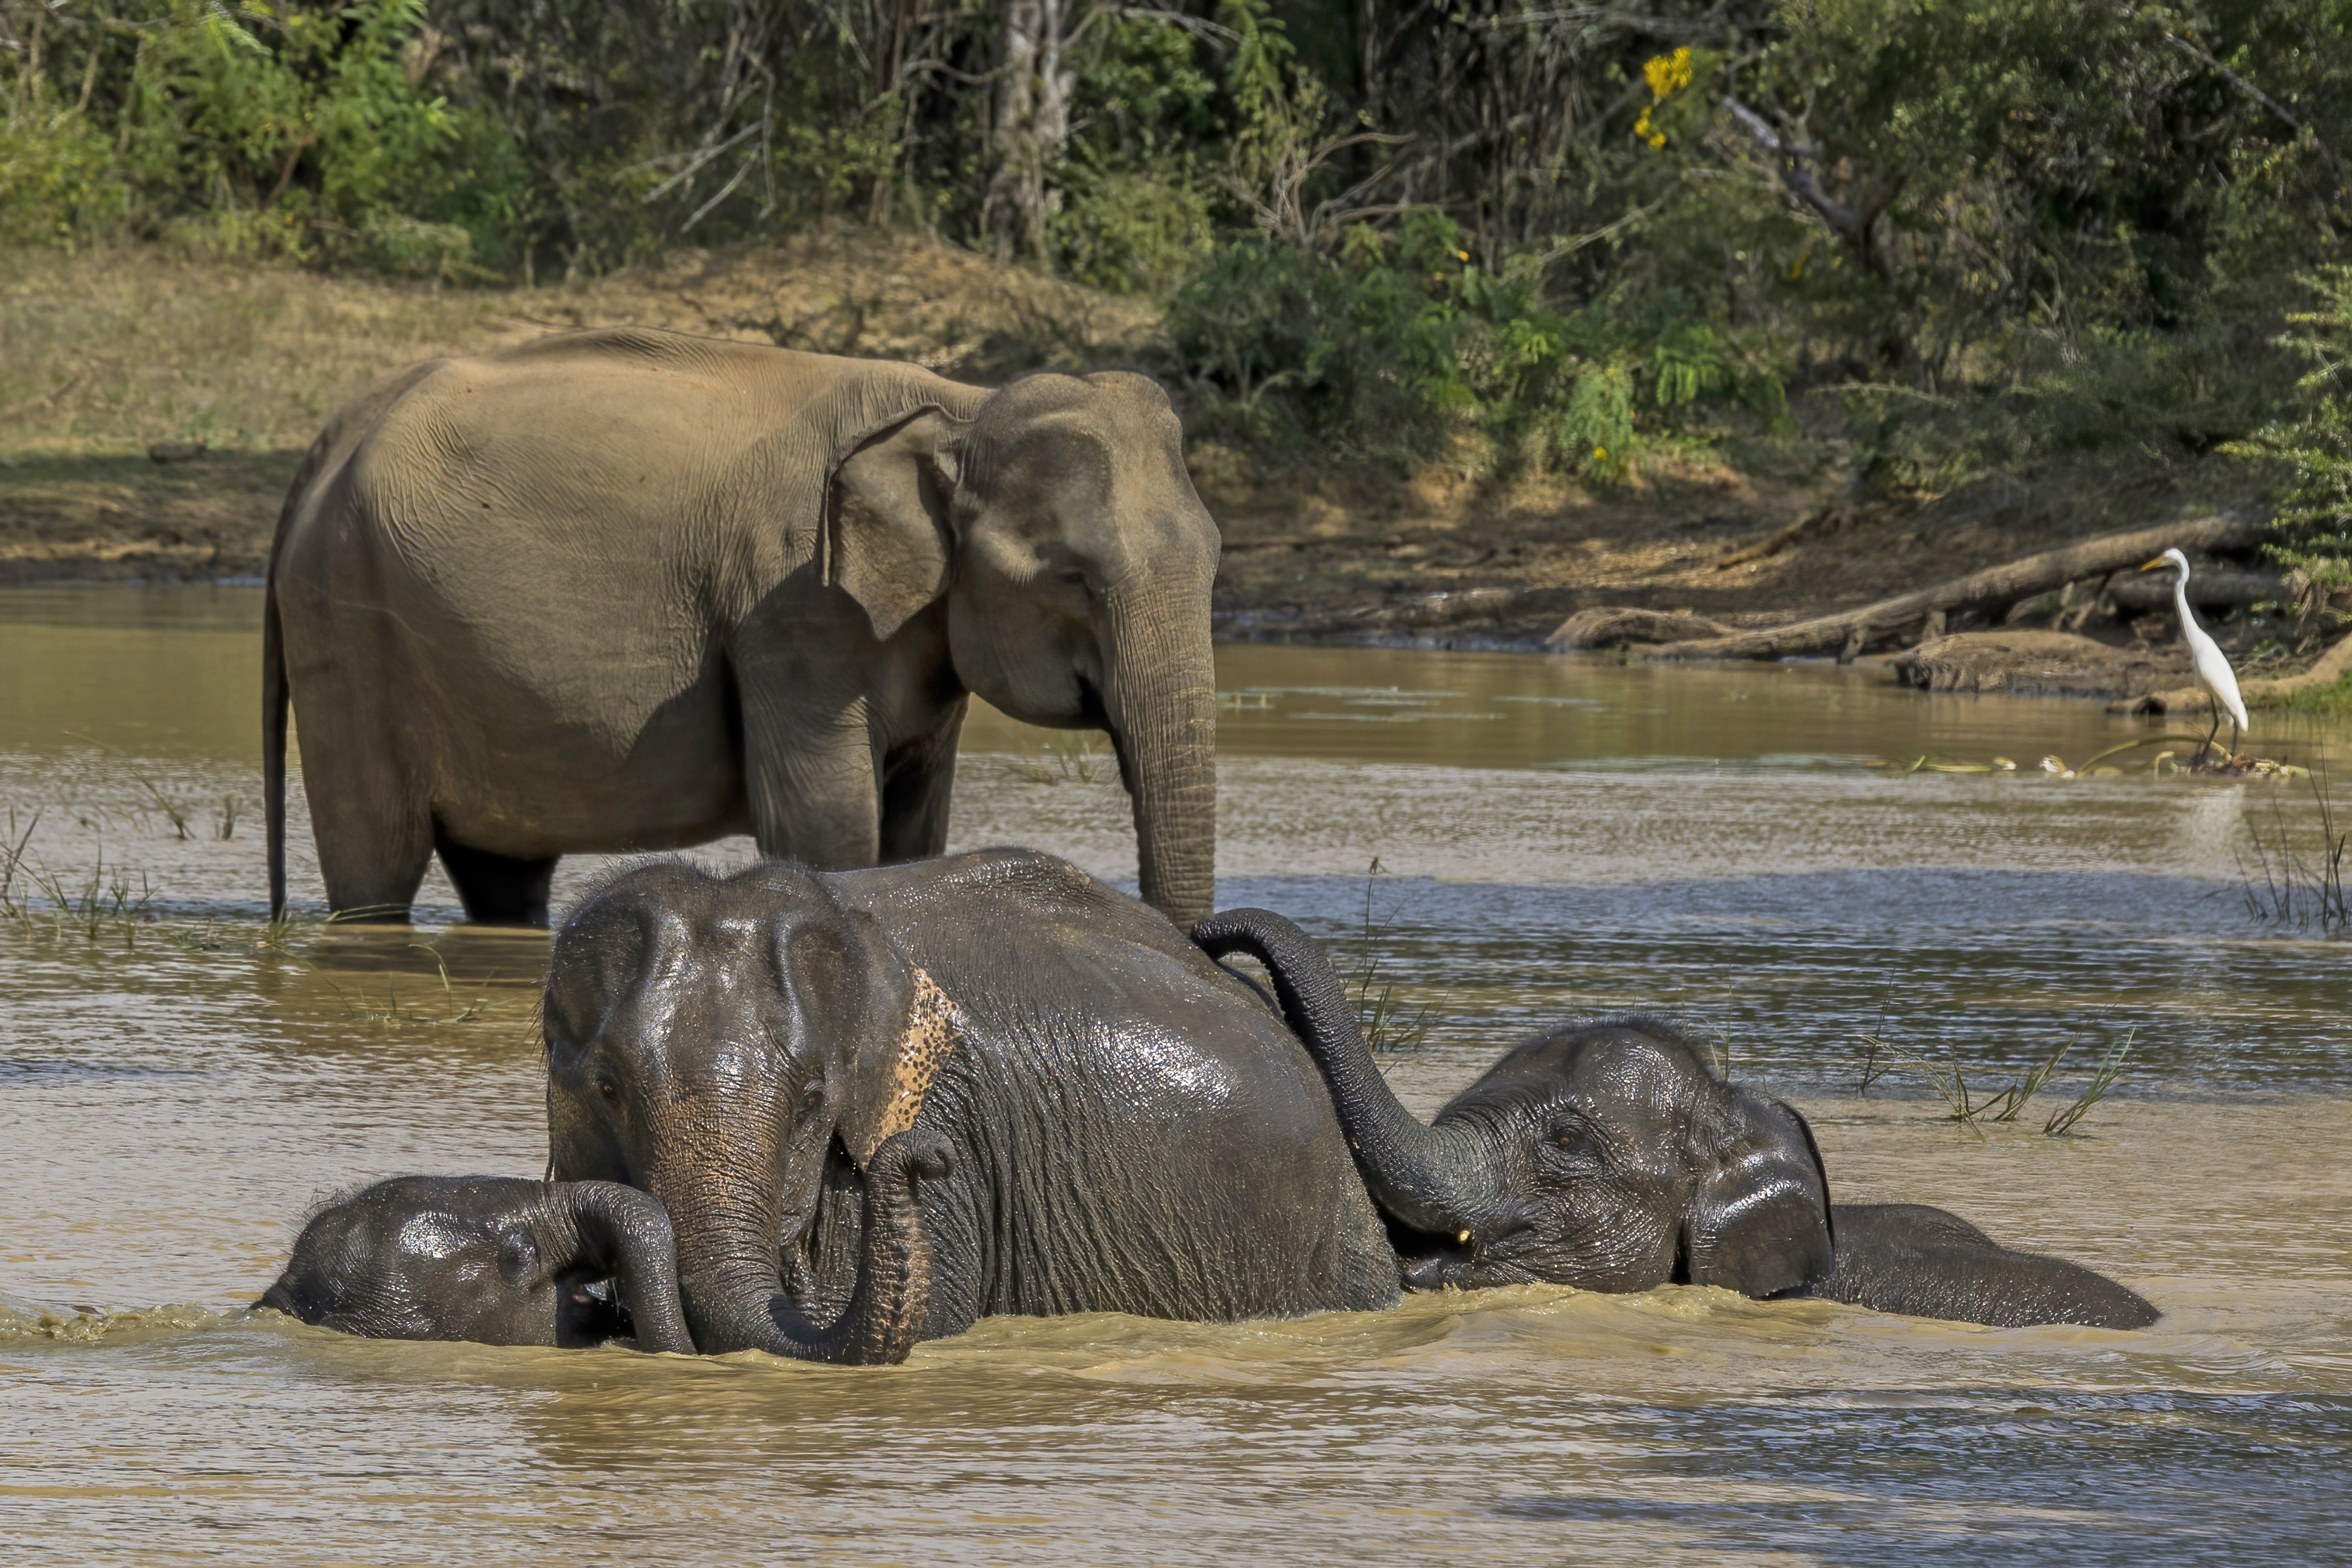
\includegraphics[width=0.9\linewidth]{elefanti.jpg}
			\end{figure}
			\scriptsize
			Source: \url{https://commons.wikimedia.org/wiki/File:Sri_Lankan_elephant_(Elephas_maximus_maximus)_female_and_young_6.jpg} \\
			Author: Charlesjsharp; Licensed under CC-BY-SA 4.0
		\end{column}
	\end{columns}
\end{frame}

\end{document}
